% !TEX root = ../report.tex
\chapter{Optimisation Results per Inflation Gas}
\label{appendix:step4-gases}

\begin{figure}[H]
  \centering
  \rotatebox{90}{%
    \begin{minipage}{0.66\textheight}
      \centering
      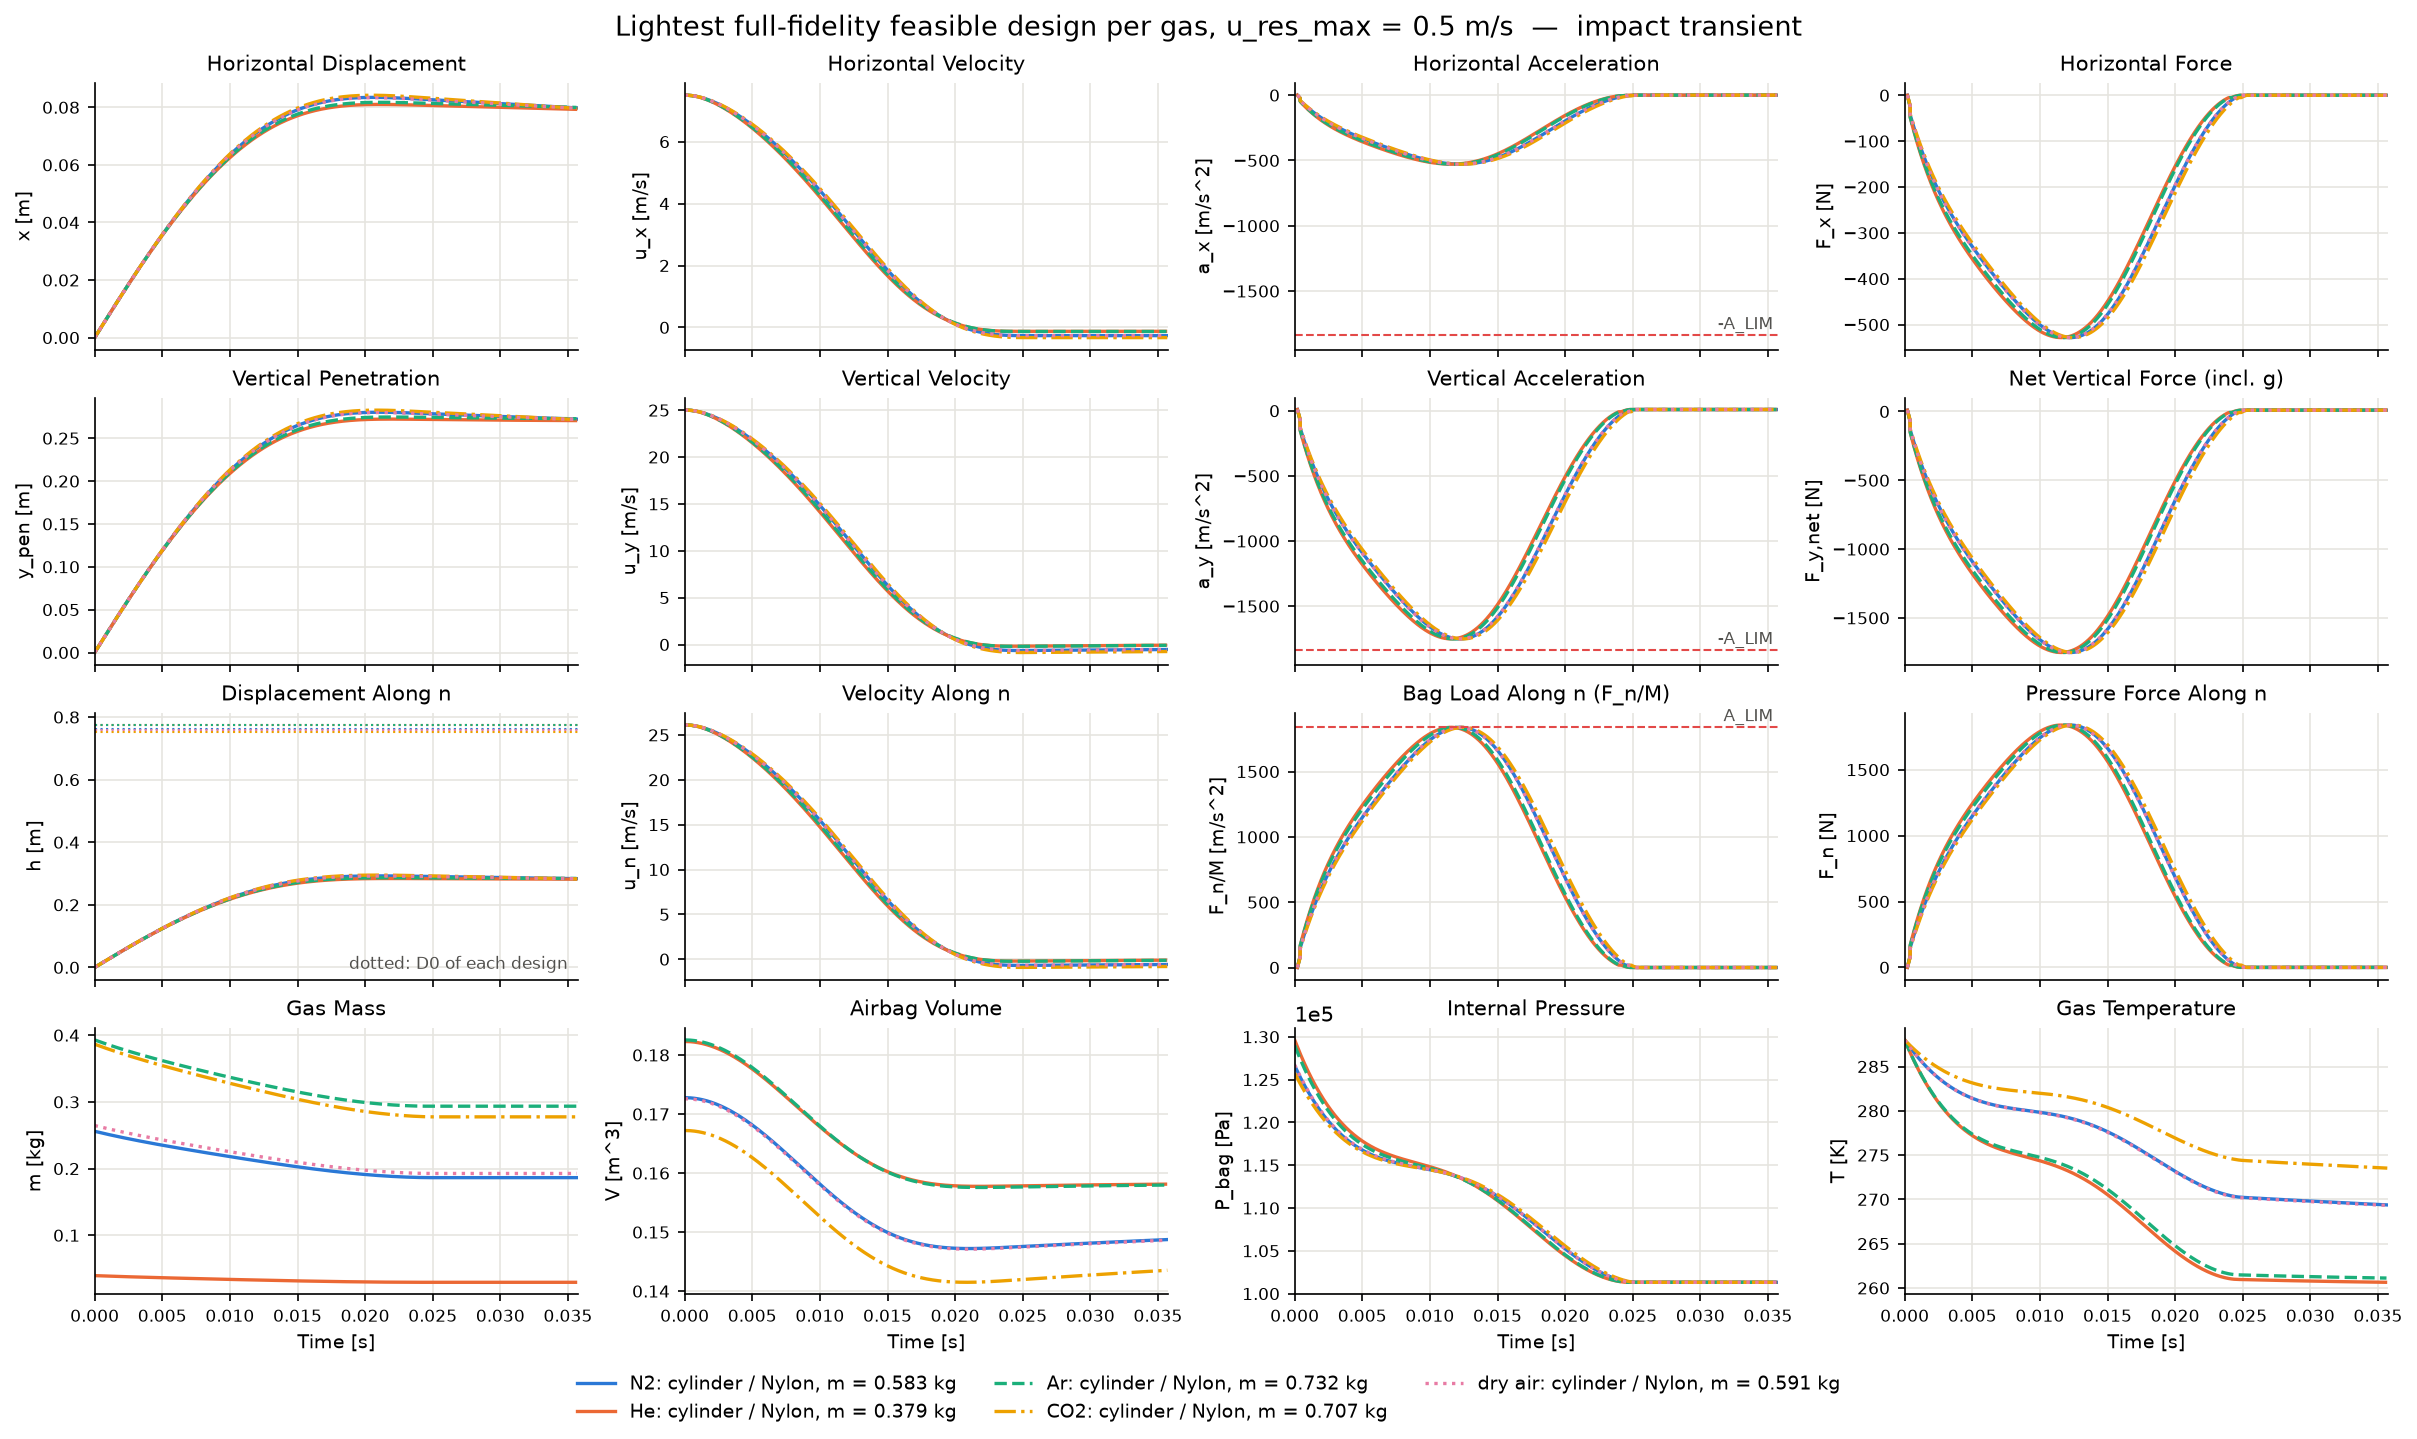
\includegraphics[width=\linewidth]{figures/chap4/step4-optimisation/overlay_gases_ures_0.5_impact.png}
      \caption{Impact transient of the lightest feasible design per inflation gas, $u_\text{res,max} = \qty{0.5}{\metre\per\second}$.}
      \label{fig:step4-gases-ures-0.5}
    \end{minipage}%
  }
\end{figure}

\begin{landscape}
\begin{figure}[p]
  \centering
  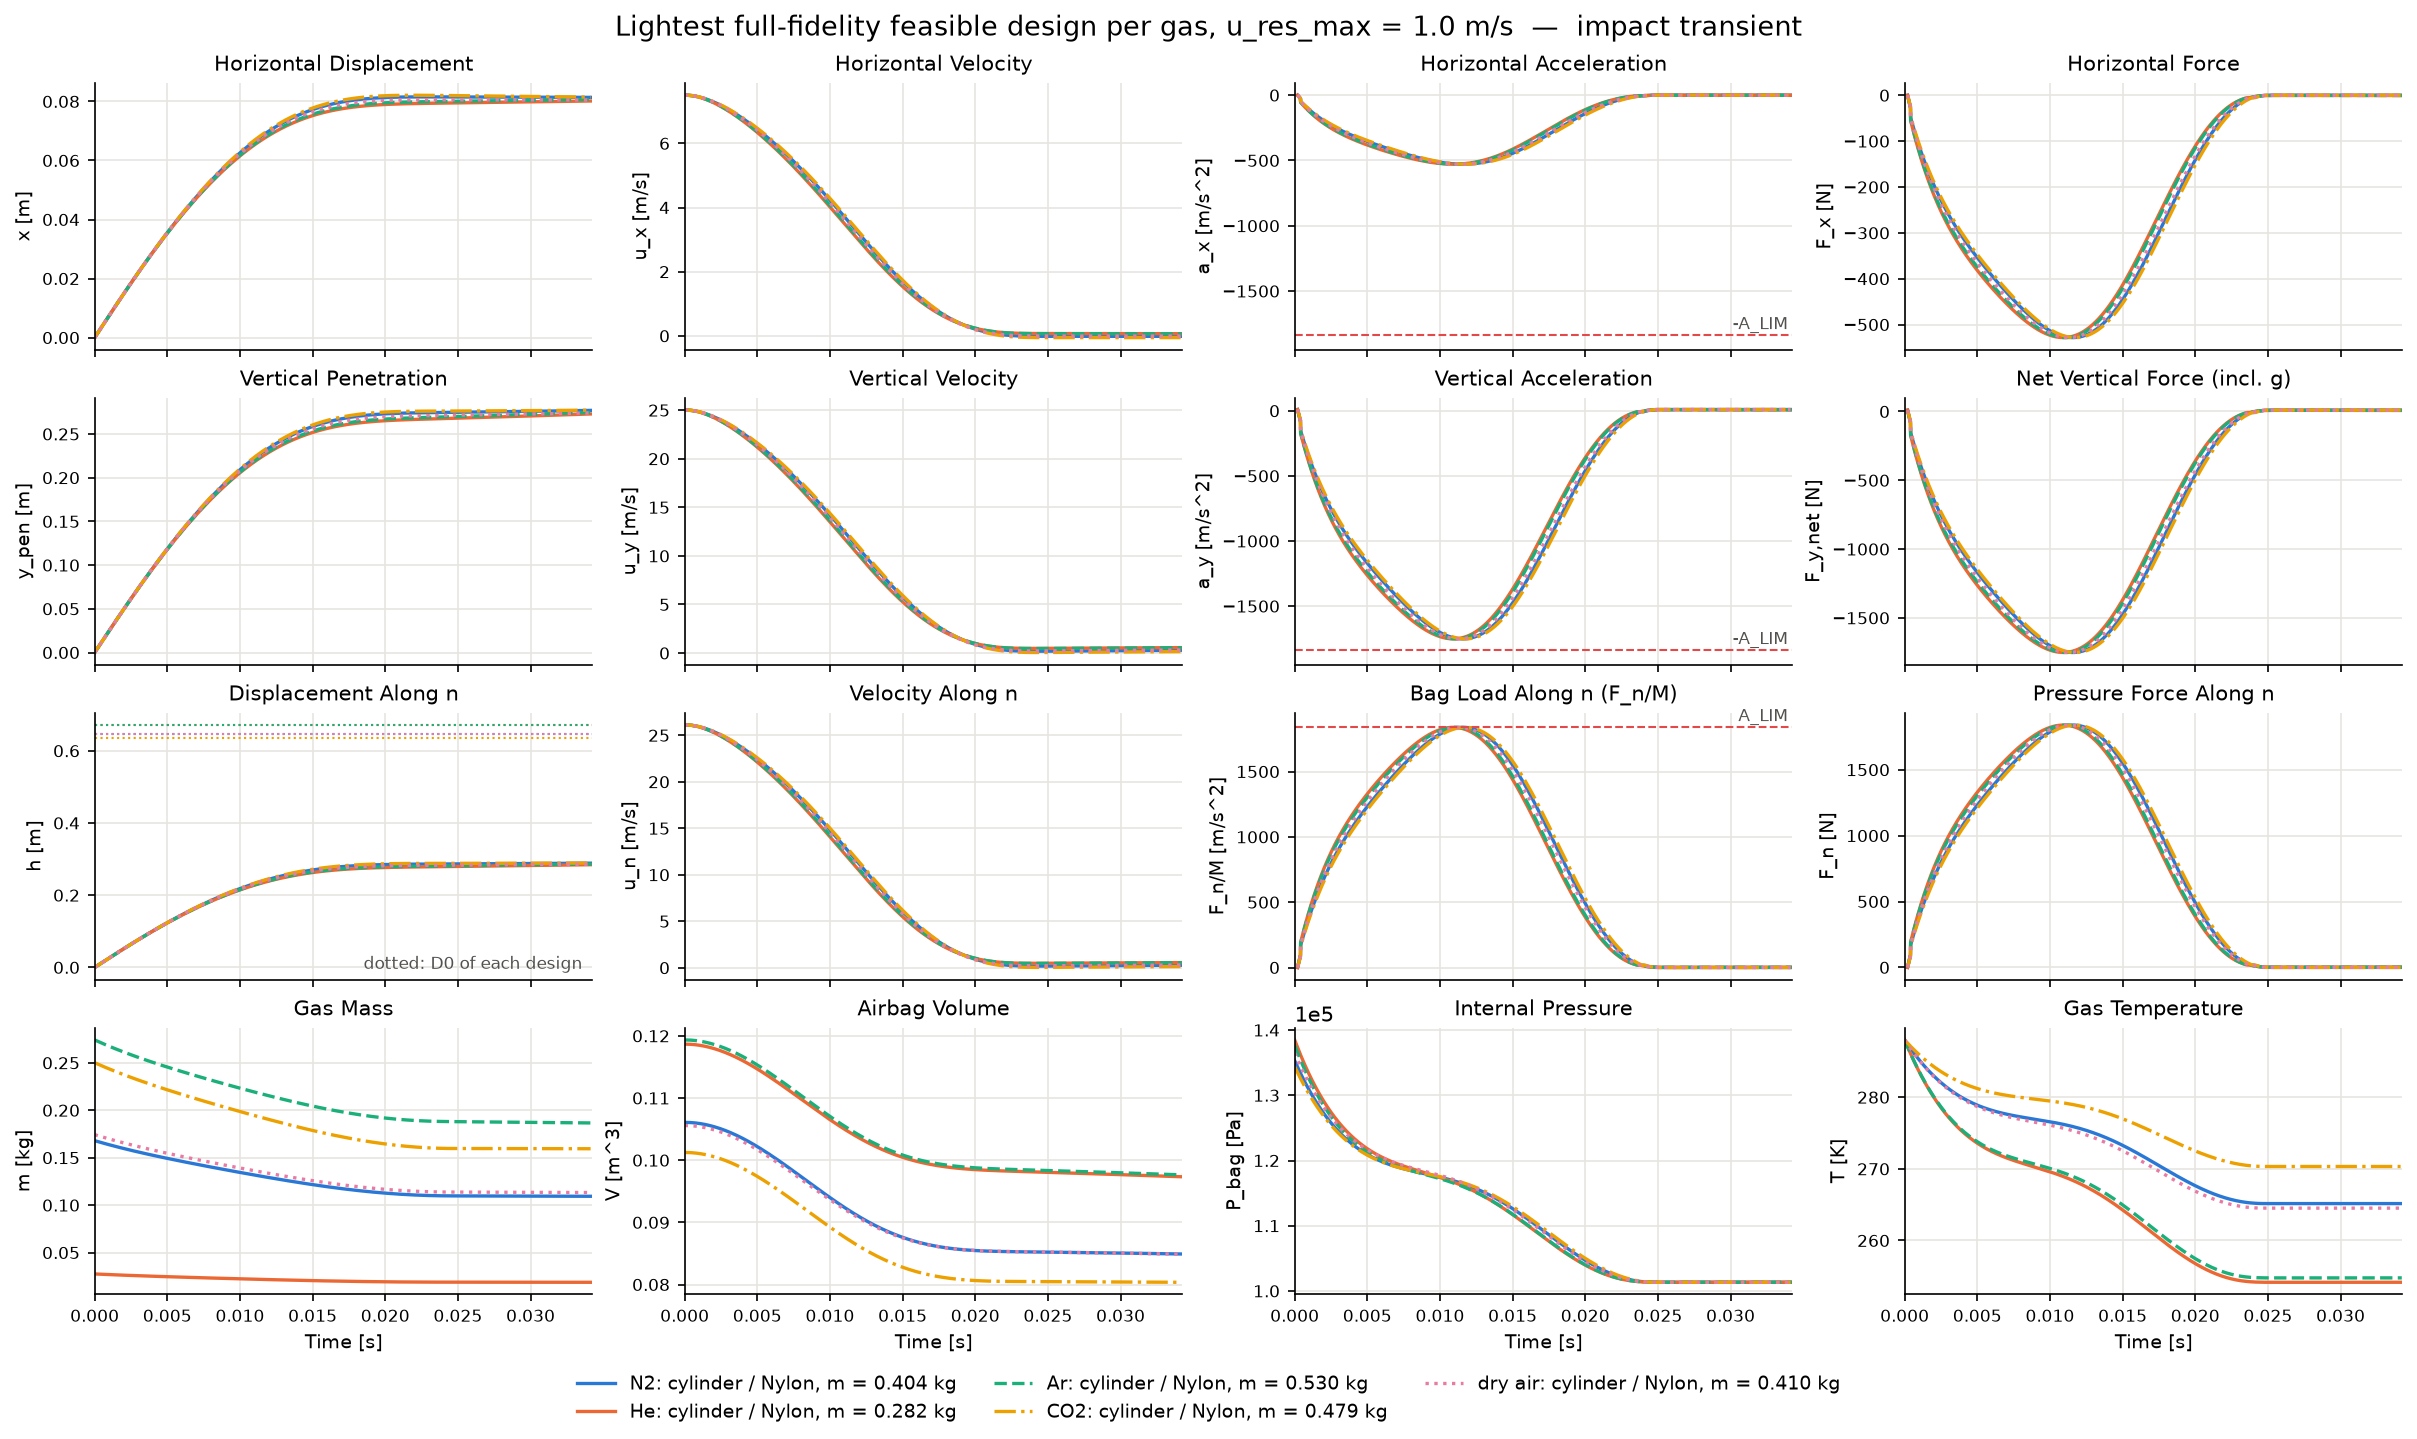
\includegraphics[width=\linewidth,height=0.85\textheight,keepaspectratio]{figures/chap4/step4-optimisation/overlay_gases_ures_1.0_impact.png}
  \caption{Impact transient of the lightest feasible design per inflation gas, $u_\text{res,max} = \qty{1.0}{\metre\per\second}$.}
  \label{fig:step4-gases-ures-1.0}
\end{figure}
\end{landscape}

\begin{landscape}
\begin{figure}[p]
  \centering
  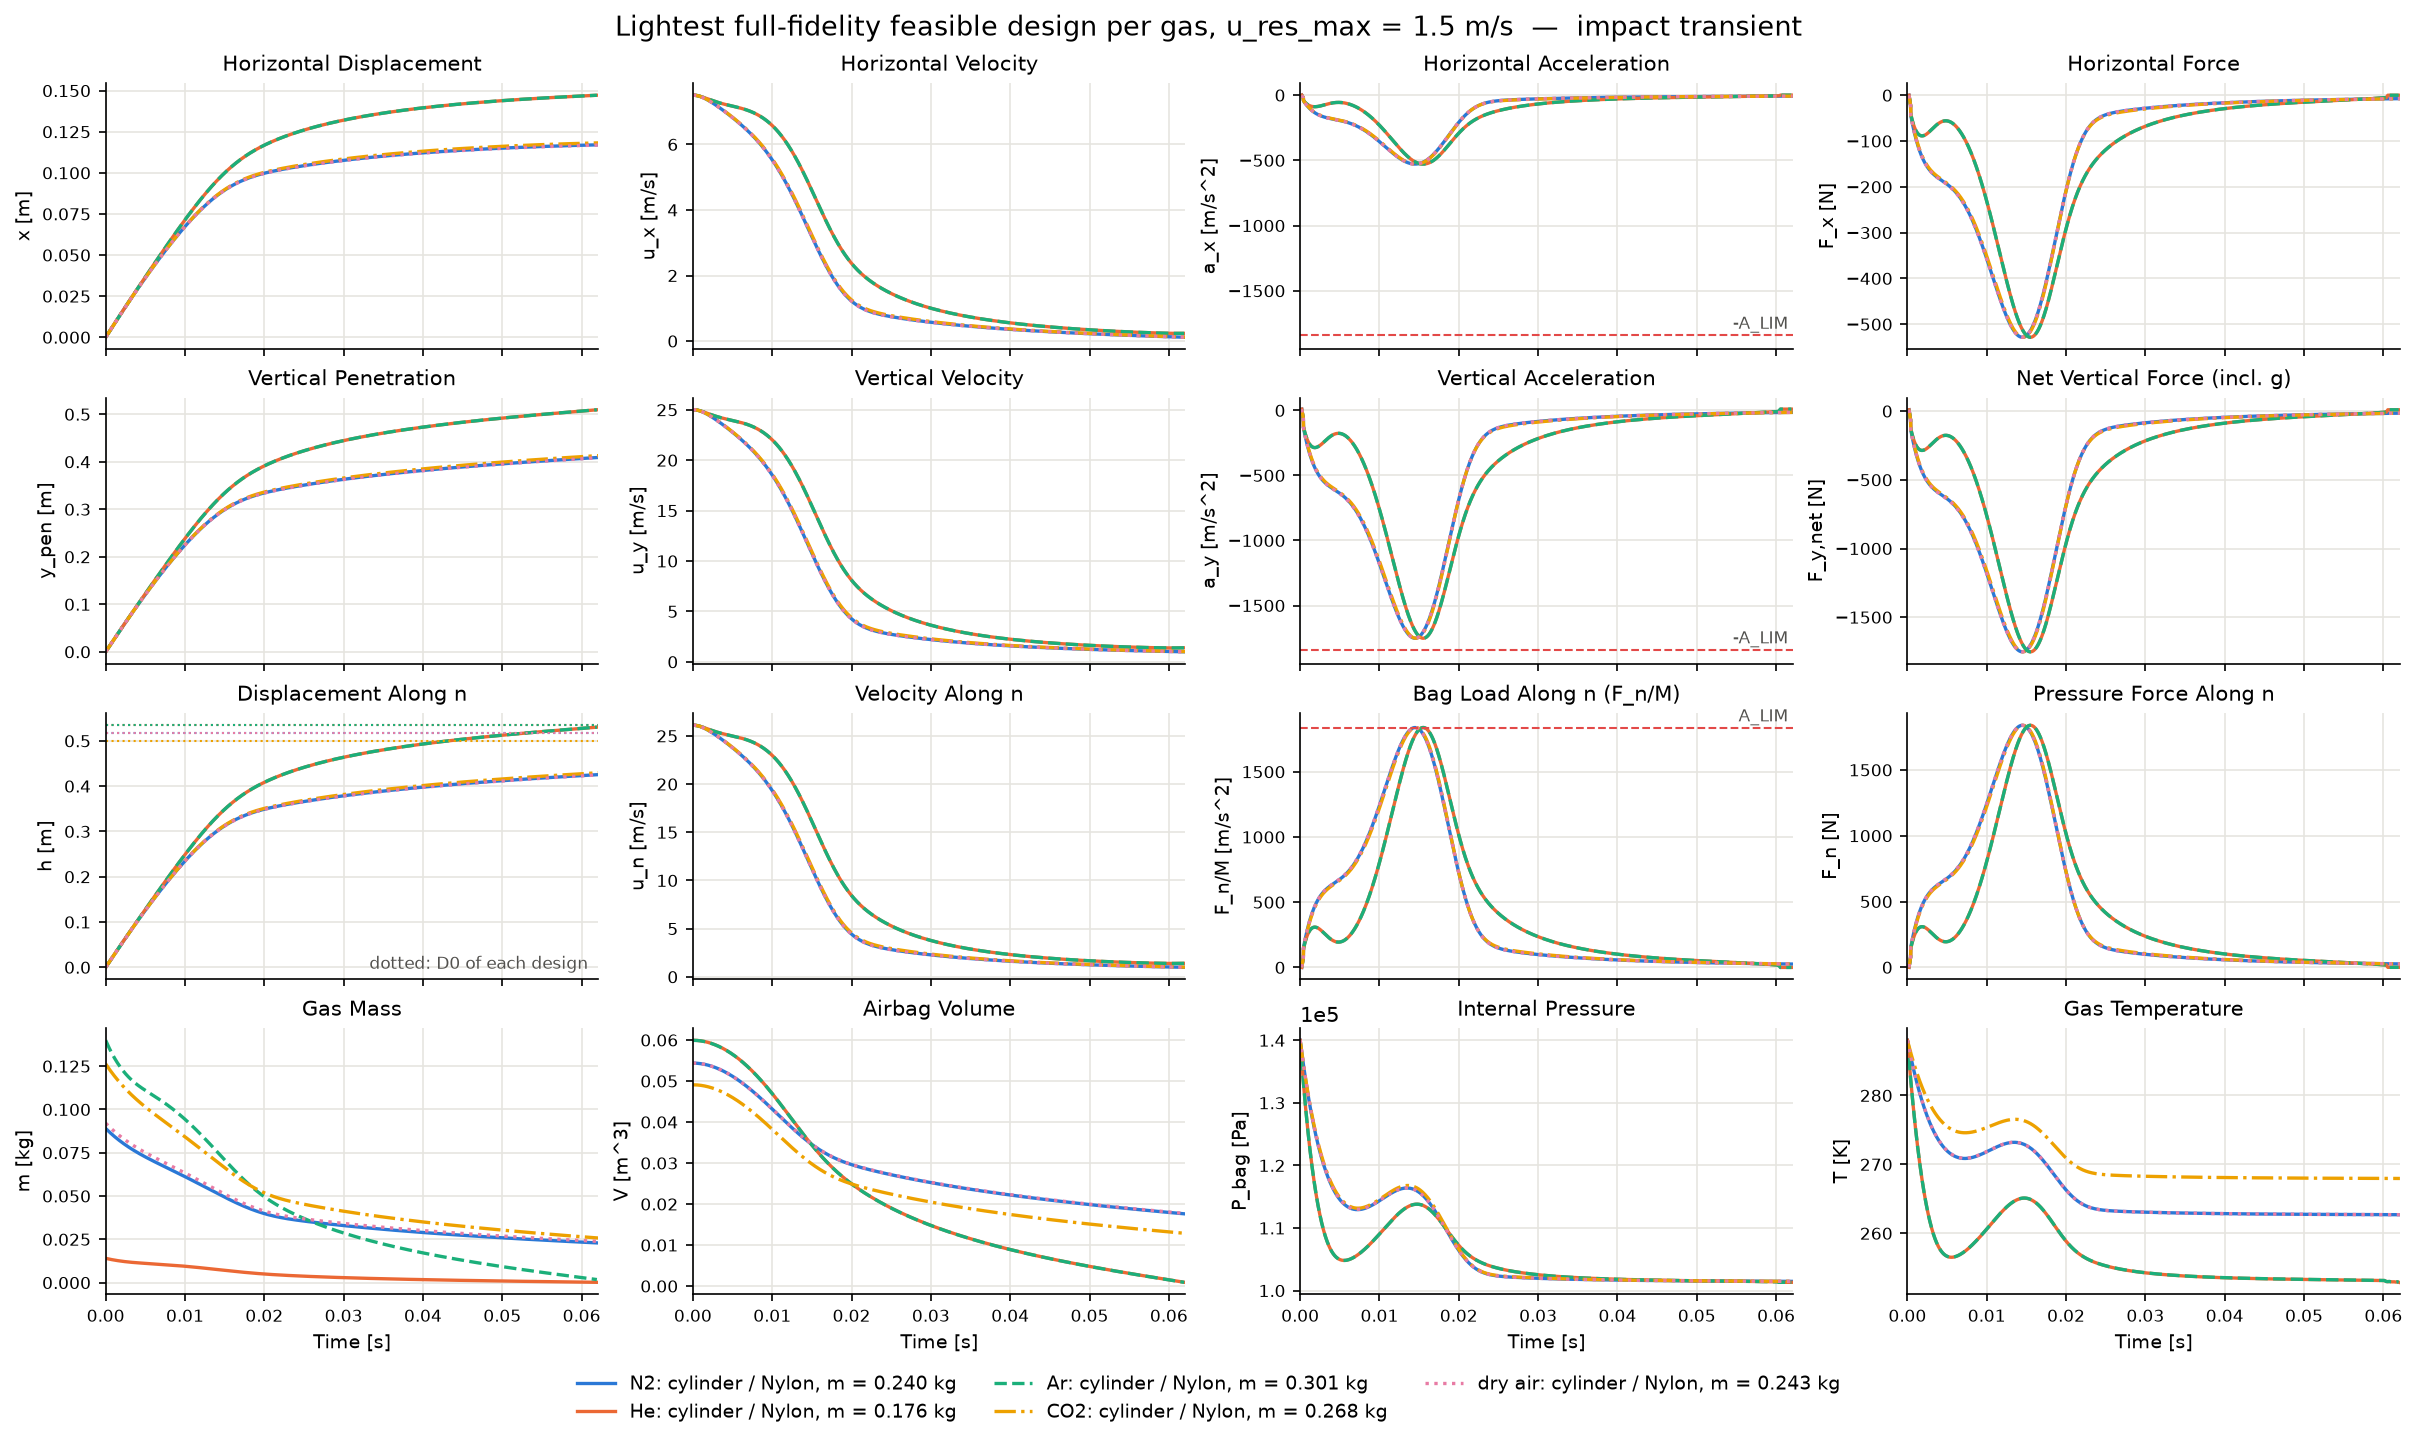
\includegraphics[width=\linewidth,height=0.85\textheight,keepaspectratio]{figures/chap4/step4-optimisation/overlay_gases_ures_1.5_impact.png}
  \caption{Impact transient of the lightest feasible design per inflation gas, $u_\text{res,max} = \qty{1.5}{\metre\per\second}$.}
  \label{fig:step4-gases-ures-1.5}
\end{figure}
\end{landscape}

\begin{landscape}
\begin{figure}[p]
  \centering
  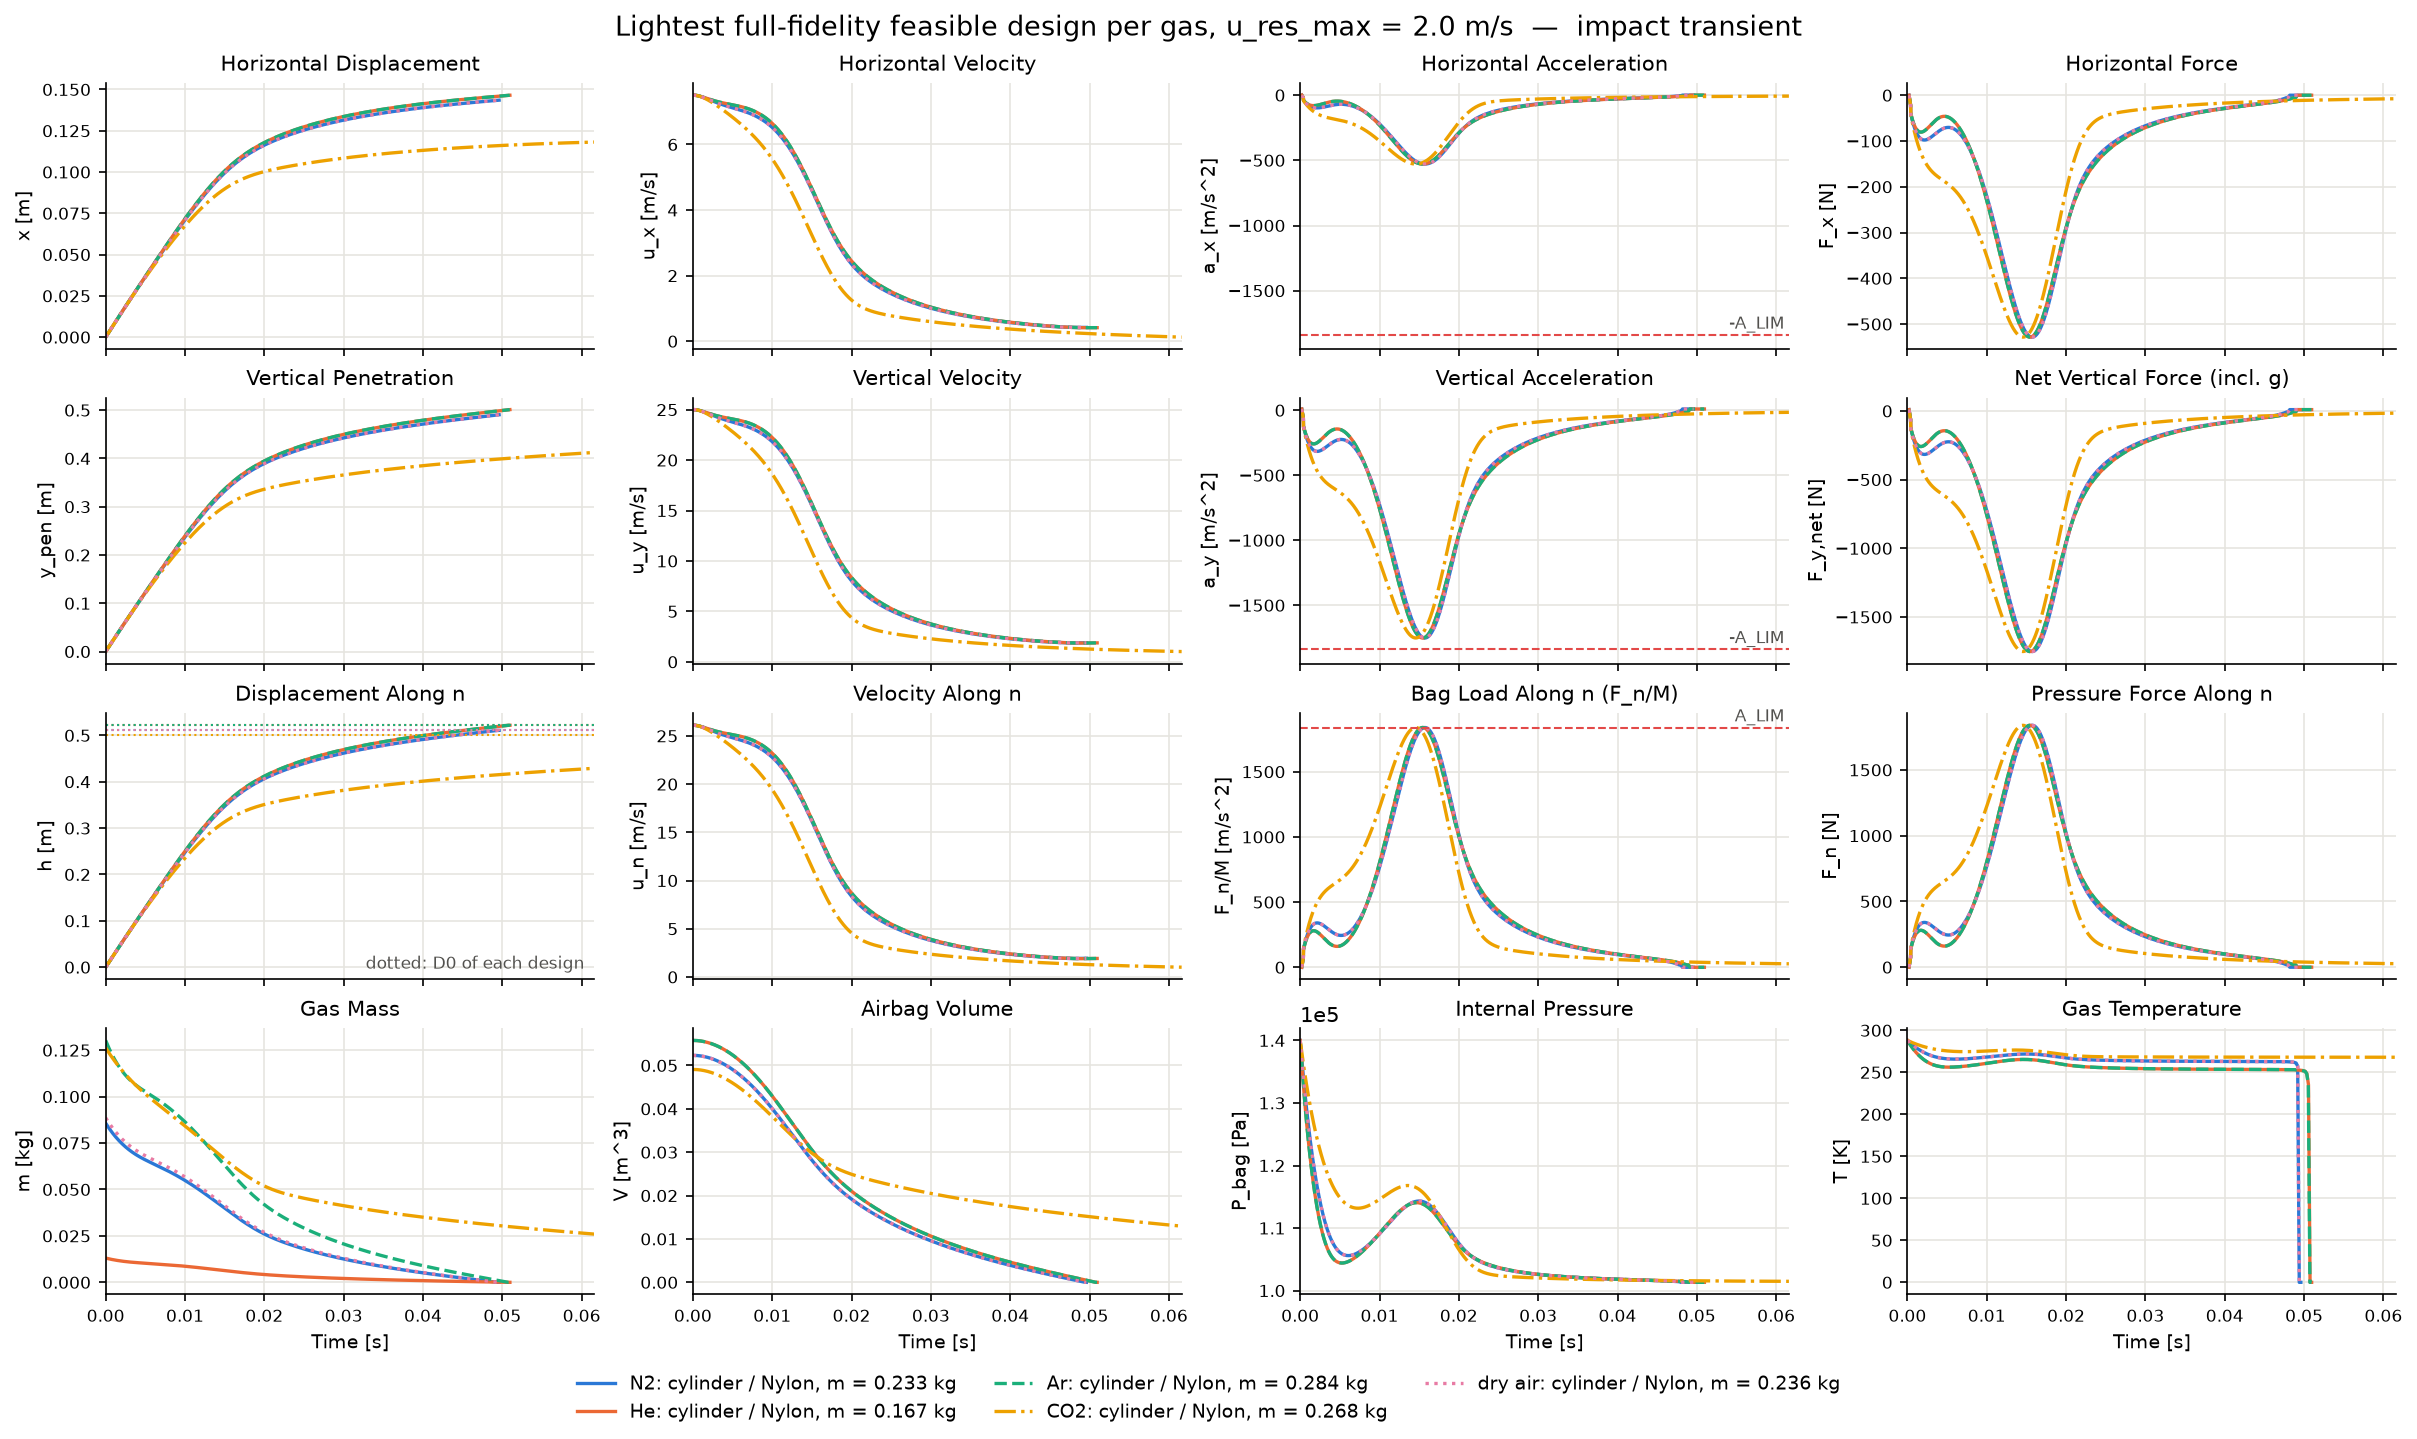
\includegraphics[width=\linewidth,height=0.85\textheight,keepaspectratio]{figures/chap4/step4-optimisation/overlay_gases_ures_2.0_impact.png}
  \caption{Impact transient of the lightest feasible design per inflation gas, $u_\text{res,max} = \qty{2.0}{\metre\per\second}$.}
  \label{fig:step4-gases-ures-2.0}
\end{figure}
\end{landscape}
